\pgfdeclarelayer{background}
\pgfdeclarelayer{beam}
\pgfsetlayers{background,beam,main}

\begin{figure}
  \centering
  \begin{tikzpicture}
    [every pin edge/.style={white,thick}]
    \begin{pgfonlayer}{background}
      \node {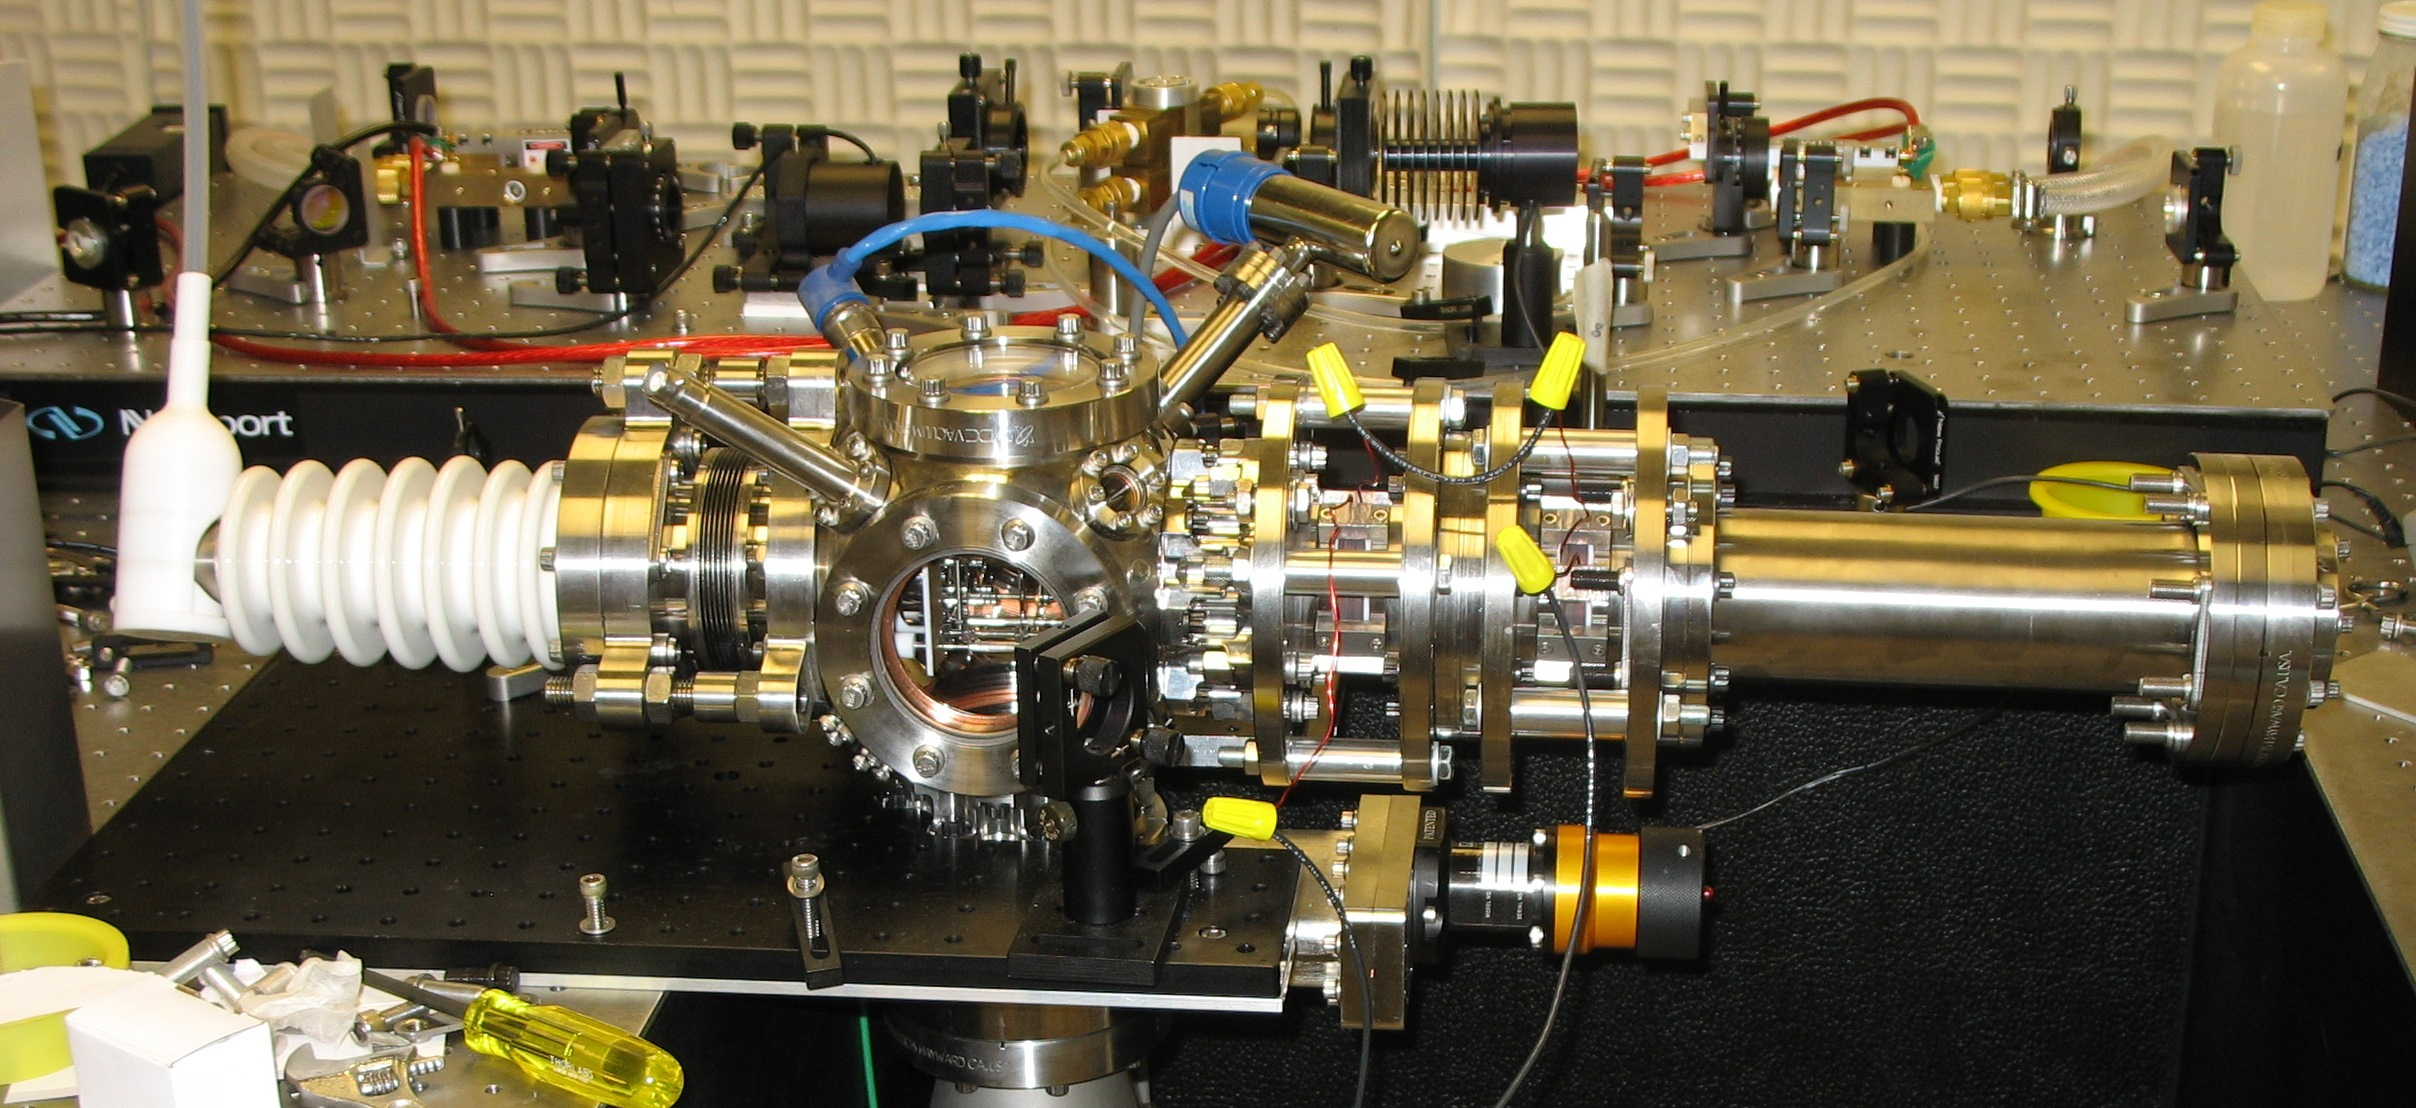
\includegraphics[width=0.9\linewidth]{column_lenses}};
    \end{pgfonlayer}
    \draw<2->
      [fill=orange] 
      (-2,-0.5)
      -- ++(0.2,0)
        node [midway,pin={below,fill=white:Photocathode}] {}
      -- ++(0,1)
        node [midway,inner sep=0.1] (source) {}
      -- ++(-0.2,0)
      -- cycle
    ;
    \draw<2->
      [fill=red]
      ($(source) + (2.35,0) $) node [inner sep=2mm] (lens1) {}
      arc (180:160:2)
      arc (20:-20:2)
        node (label lens1) {}
      arc (200:180:2)
    ;
    \draw<2->
      [fill=red]
      ($(source) + (3.4,0) $) node [inner sep=2mm] (lens2) {}
      arc (180:160:2)
      arc (20:-20:2)
        node (label lens2) {}
      arc (200:180:2)
    ;
    \node<2-> at ($(lens1)!0.5!(lens2) + (0,-1.5)$) (lens label) [red,fill=white] {Magnetic Lenses};
    \foreach \x in {1,2}
      \draw<2-> [white,thick] (lens label) -- (label lens\x);
    \draw<2-> 
      [fill=green!40]
      ($(source) + (6.5,0)$) node [inner sep=0] (detector) {}
        ellipse (0.2 and 0.5) 
          node at ($(source) + (6.5,-0.5)$) [pin={below,fill=white:Detector}] {}
    ;
    \draw<3->
      [green,very thick]
      (-5.2,-0.7)
      -- (-0.7,-0.7)
        node [pos=0.2,below=2mm,fill=white] {Laser}
      -- (source.east)
    ;
    \draw<5-> [fill=gray!60]
      ($(lens1)!0.5!(lens2) + (-0.05,0.5)$)
      node [pin={above,fill=white:{RF Cavity}}] {}
      rectangle ++(0.3,-1)
    ;
    \begin{pgfonlayer}{beam}
      \fill<4->
        [blue!40]
        (source)
        -- (lens1.north)
        -- (lens2.north)
        -- (detector.east)
          node [midway,above=5mm,fill=white] {Electron Beam}
        -- (lens2.south)
        -- (lens1.south)
      ;
    \end{pgfonlayer}
  \end{tikzpicture}
\end{figure}
